\chapter*{Succeeding with Agile}

\ifnotes

\fi

\ifcontent

    \section*{Isn't "Agile" enough?}
    
    Agile methods, in the simplest terms, work by requiring three things:
    
    \begin{enumerate}
        \item Working in small increments
        \item Getting frequent feedback
        \item A focus on technical excellence
    \end{enumerate}
    
    \QandAbox{Why do things still go wrong?}{2}
    
    \section*{Shifting left}
    
    \begin{framed}
        If you make an requirements error and find it during the requirements phase it is inexpensive to fix. In the design stage, it is more expensive to fix ... in the order of 10x. During programming the cost is in the order of 100x. If you find the error during testing stage, it is in the order of 1,000x to fix. Finally, if the error gets into production, you are looking at cost of 10,000x to fix

       \begin{flushright}
            \textit{Scott W. Ambler}
        \end{flushright}
    \end{framed}
    
    
    Label the axes and draw a curve that represents Ambler's statement on the graph below:
    
    \begin{center}
        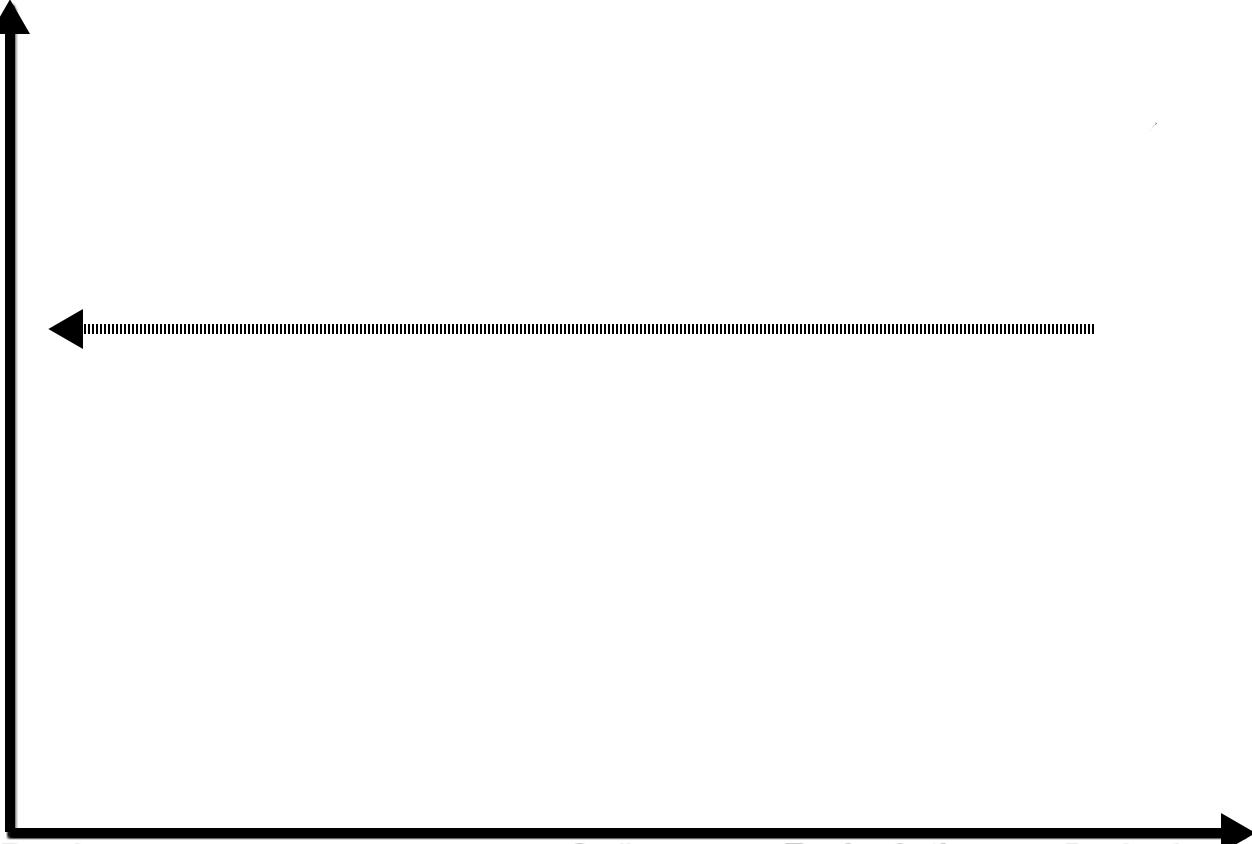
\includegraphics[height=8cm, keepaspectratio]{images/shift-left-axes}
    \end{center}

    
    \section*{How can we test earlier?}

    \begin{framed}
       "[Testing is] the process of gathering information about something with the intent that the information could be used for some purpose." 
       
       \begin{flushright}
            \textit{Jerry Weinberg, Perfect Software (and Other Illusions About Testing)}
        \end{flushright}
    \end{framed}    

    \QandAbox{What can we test before any code is written?}{8}
    
    \QandAbox{What common problems do teams experience if they leave testing till late in the software development process}{4}
    
\fi